%*
%* Seven Kingdoms: Ancient Adversaries
%*
%* Copyright 1997,1998 Enlight Software Ltd.
%* Copyright 2018 Timothy Rink
%*
%* This program is free software: you can redistribute it and/or modify
%* it under the terms of the GNU General Public License as published by
%* the Free Software Foundation, either version 2 of the License, or
%* (at your option) any later version.
%*
%* This program is distributed in the hope that it will be useful,
%* but WITHOUT ANY WARRANTY; without even the implied warranty of
%* MERCHANTABILITY or FITNESS FOR A PARTICULAR PURPOSE.  See the
%* GNU General Public License for more details.
%*
%* You should have received a copy of the GNU General Public License
%* along with this program.  If not, see <http://www.gnu.org/licenses/>.
%*
%*

\chapter{Starting a New Game}

\index{getting started}
\index{starting a game} % Expand?

\section{Installation and Start-up}

\index{game!installation}
\index{installation}

\subsection{Minimum Requirements}

\index{game!system requirement}
\index{system requirements}

\textgoth{\Huge{T}}o play \textit{Seven Kingdoms: Ancient Adversaries}, the following hardware and software is required:

\begin{itemize}
	\item x86 or x86\_64 little-endian processor, Pentium or better
	\item SDL2.0 with accelerated OpenGL or DirectX compliant video drivers
	\item 32 MB of RAM
\end{itemize}

\subsubsection{Optional Requirements}

\index{network play}
\index{playing on a network}

\begin{itemize}
	\item IPv4 UDP connection for LAN and Internet play
\end{itemize}

\subsection{Download}

\textit{\textgoth{\Huge{S}}even Kingdoms: Ancient Adversaries} can be downloaded at the Download page of the Wiki on the 7kfans.com website. Select the version you want to install. Then, launch the installer to begin.

\subsection{License}

\textgoth{\Huge{M}}ost of the assets for \textit{Seven Kingdoms: Ancient Adversaries} is provided through the GPLv2 License. With the GPLv2 you have: 

\begin{itemize}
	\item the freedom to run the program as you wish, for any purpose.
	\item the freedom to study how the program works, and change it so it does your computing as you wish. 
	\item the freedom to redistribute copies so you can help your neighbor.
	\item the freedom to distribute copies of your modified versions to others, providing you keep the same GPLv2 license terms in the copies you distribute.
\end{itemize}

\textbf{Note:} the music is not GPL or public domain. The music may not be modified or re-recorded. The music author allows the music tracks may be freely provided with the game, and granted no other rights.

\subsection{Select Components to Install}

\subsubsection{Music}

You may choose to install the music or not. It is 49.3 MB.

\subsubsection{OpenAL}

OpenAL is a cross-platform audio application programming interface. It is not necessary to install if you already have an equivalent driver, such as DirectX, etc.

\subsubsection{Start Menu Shortcuts}

You may choose to install start menu shortcuts or not. Regardless, a desktop shortcut will be installed.  

\subsection{Directories}

\textgoth{\Huge{A}}t this portion, you may choose folder options, such as:

\begin{itemize}
	\item Choosing the destination folder for install.
	\item Choosing start menu folder or name, and if you still want to install the start menu shortcuts.
\end{itemize}

\subsection{Updates}

\textgoth{\Huge{K}}eep an eye on the Experimental Builds thread on the forums for announcements regarding updated Windows binaries. These development releases tend to have bug fixes or additional features. Or visit the Download page to see if an update has been released.

\subsection{Start up}

\index{game!starting}

\textgoth{\Huge{L}}aunch 7kaa.exe to begin playing by \textbf{Clicking} on the \textit{Seven Kingdoms: Ancient Adversaries} icon. If you chose to install the start menu shortcuts in Seven Kingdoms AA or a folder of your choosing, you may also start it from there. \\ % Adds vspace for the graphics.


\includegraphics[width=0.07\linewidth]{7kicon} % The only color graphic here.

\clearpage % keep here.

\section{The Main Menu}

\index{main menu}

\textgoth{\Huge{Y}}our entrance to the world of \textit{Seven Kingdoms: Ancient Adversaries} begins.

\begin{wrapfigure}{r}{0.5\textwidth}
	\begin{center}
		\vspace{-20pt}
		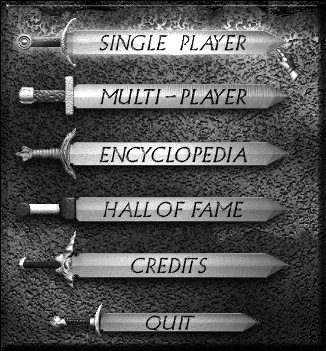
\includegraphics[width=0.4\textwidth]{SWmainmenu}
	\end{center}
	\vspace{-20pt}
\end{wrapfigure}

You will be taken to the Main Menu, where you will have a choice between playing a Single-Player or Multi-Player Game, or viewing the Encyclopedia or Hall of Fame. You also have the option to quit.

\subsection{Single-Player Game}

\index{game!single-player}
\index{single player game}

\textgoth{\Huge{I}}f you want to play a Single Player Game, \textbf{Click} on the Single Player Sword. When you do, you will bring up the following menu: 

\begin{center}
	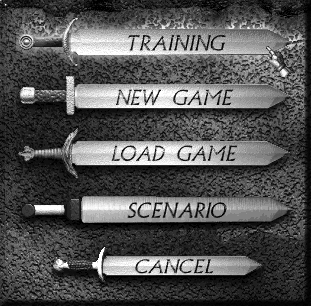
\includegraphics[width=0.5\linewidth]{SWsingleplayer}
\end{center}

\clearpage

\subsubsection{Training}

\index{game!training}
\index{training}

\textgoth{\Huge{I}}t is \textbf{\textit{strongly}} recommended that new players begin with the Training section. You may wish to go through all of the Training sessions even before reading the rest of this manual, which has been designed as an in-depth reference book.

When you \textbf{Click} on the Training Sword, you will be taken to a menu listing all of \textit{Seven Kingdoms: Ancient Adversaries} Training lessons.

\begin{center}
	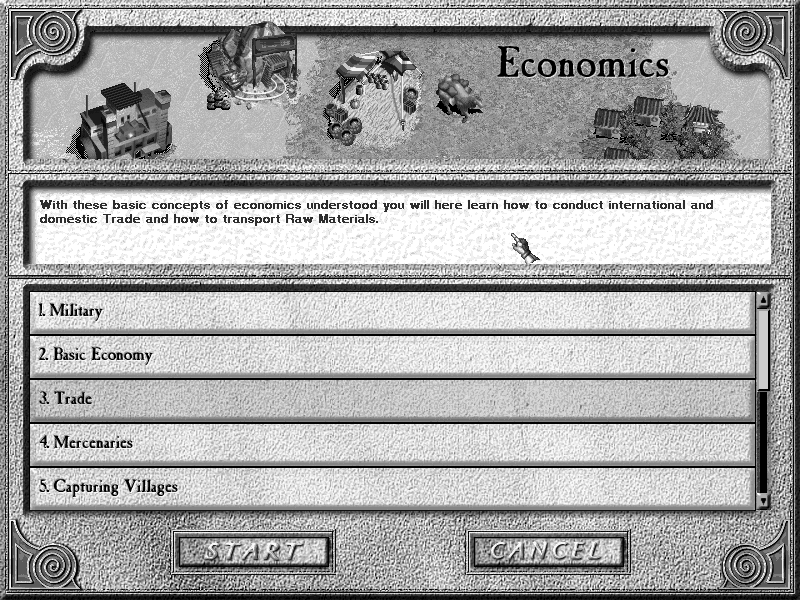
\includegraphics[width=0.9\linewidth]{Itraining}
\end{center}

\textbf{IMPORTANT}: It is best if you take these lessons in order as later lessons will assume that you understand concepts presented previously.

When you \textbf{Click} on a topic you will see a brief description of the lesson. If you decide to proceed with the selected lesson, \textbf{Click} on the \textbf{Start Button}.

This will load a predesigned training scenario that will correspond to the chosen lesson.

The lesson text will appear at the top of your screen, leaving plenty of space for you to control the game below.

\begin{center}
	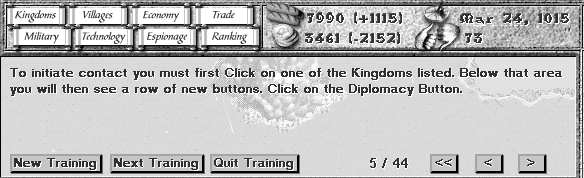
\includegraphics[width=0.9\linewidth]{Ilesson}
\end{center}

Page though the lessons by \textbf{Clicking} on the \textless and \textgreater \hspace{1pt} \textbf{Buttons} or do the same by pressing your \textless and \textgreater keys on your keyboard.

It is not strictly necessary that you learn your lessons within the designated training scenario. At any time during any Single Player game you may load a Training lesson if you wish to review any aspect of the game.

If you wish to proceed to the next lesson while remaining in the same game, \textbf{Click} on the \textbf{Next Training Button}.

To select a lesson that may not be the next in the series, \textbf{Click} on the \textbf{New Training Button}. This will return you to the menu where you can preview and select a different lesson.

\subsubsection{New Game}

\index{game!starting}
\index{new game}

\textbf{\textgoth{\Huge{C}}licking} on the New Game Sword will take you to the New Single Player Game options screens. Here you will see the four following Options pages:

\begin{center}
	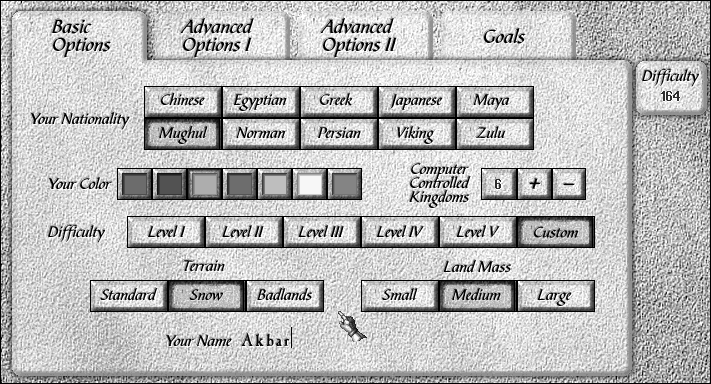
\includegraphics[width=0.9\linewidth]{Ibasicoptions}
\end{center}

On the \textbf{Basic Options} page, you may set your choices for your nationality, color, and the number of computer players.

Other options are also available below. Choose the level of difficulty at which you wish to play and then \textbf{Click} on that button. Level I is the generally the easiest and Level V the most difficult. Setting a level will automatically set corresponding options on the following Advanced Options I and II pages.

The final button, Custom, will be automatically set if you choose any options that do not match with the preset difficulty levels.

Two more options on this page are Terrain style and Land Mass. You will have three choices for each.

On the far right you can see an area with a number labeled “Difficulty”. This number will rise or fall depending upon the options that you set for the game. The maximum difficulty possible is 200. This difficulty number will be used to determine your final score---a higher difficulty rating means that the possible range of scores will be higher as well.

On the bottom of this options page there is space for you to type in your name. This name will be used by your King at the start of the game.

On the \textbf{Advanced Options I} page you will find the following options:

\begin{center}
	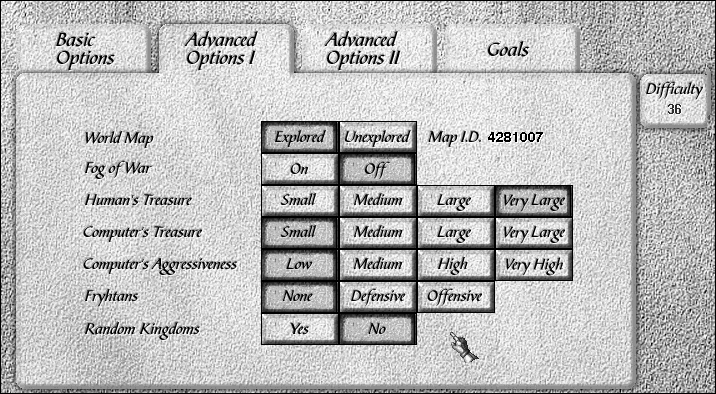
\includegraphics[width=0.9\linewidth]{Iadvancedoptions1}
\end{center}

\textbf{World Map}: Here you may choose whether the world will be unexplored at the start of the game, or completely explored with all map features visible.

\begin{changemargin}{0.5cm}{0cm} 
 \textbf{The Map I.D.} is the random-number seed from which your new world map will be generated. If you wish to play with a map that you particularly enjoyed from a previous game, you may enter its number by typing it in on your keyboard. Do not enter the commas that separate the numbers. They are there to make the number easier to read.
\end{changemargin}

\begin{changemargin}{0.5cm}{0cm} 
 If you have already begun a game and wish to check on the Map I.D., \textbf{Click} on the \textbf{Menu Button} at the top right of your screen. The Map I.D. will be on the bottom of the Menu area.
\end{changemargin}

\textbf{Fog of War}: Here you decide whether there is a limit to the distance your units can see (On) or if you will be able to see all activity in the world at any time (Off).

\textbf{Human’s Treasure}: Sets the amount of money with which you will begin the game.

\textbf{Computer’s Treasure}: Sets the amount of money with which your computer foes will begin the game.

\textbf{Computer’s Aggressiveness}: Sets whether your computer-controlled rivals are passive or aggressive.

\textbf{Fryhtans}: This will determine if Fryhtans are a part of the game or not, and if they are, whether they will only fight to defend themselves, or if they may attack on their own initiative.

\begin{changemargin}{.5cm}{0cm}
If set to Defensive, the Fryhtans will remain in their Lairs unless attacked.

If set to Offensive, Fryhtans may attack on their own, especially if a village is settled or a building built too near to their Lair. 

They will also expand their numbers by planting new Lairs around the land.
\end{changemargin}

\textbf{Random Kingdoms}: When this option is turned On, the computer will randomly choose the nationalities of other Kingdoms in the game. It is quite possible, in this case, that other Kingdoms will be of the same nationality as your own. This can make for very interesting games as you vie for control of Independent Villagers who share your nationality.

This setting will also randomize each Kingdom’s initial Village population, including your own. A small population will be somewhat offset by granting a few skilled, mobile units at the start of the game.

\begin{center}
	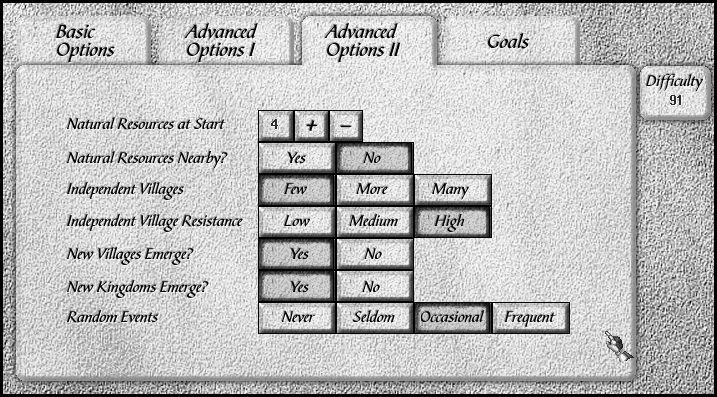
\includegraphics[width=0.9\linewidth]{Iadvancedoptions2}
\end{center}

On the \textbf{Advanced Options II} page you will find still more options. These are as follows:

\textbf{Natural Resources at Start}: This number, between 1 and 7, will set how many Natural Resources will be spread throughout the world at the start of the game.

\textbf{Natural Resources Nearby?}: This option determines whether or not each kingdom will have a Natural Resource deposit automatically located near its starting village.

\textbf{Independent Villages}: This sets the approximate number of Independent Villages.

\textbf{Independent Village Resistance}: This sets the level of resistance to your rule for all of the Independent Villages. It also influences the Combat abilities of Independent units.

\textbf{New Villages Emerge?}: This determines whether or not new Independent Villages may be settled during the game.

\textbf{New Kingdoms Emerge?}: This determines whether or not new Kingdoms may be founded after the destruction of old ones.

\textbf{Random Events}: This sets the frequency of random natural disasters such as earthquakes, lightning strikes, and tornadoes---all of which can cause damage to buildings and injury to units.

\begin{center}
	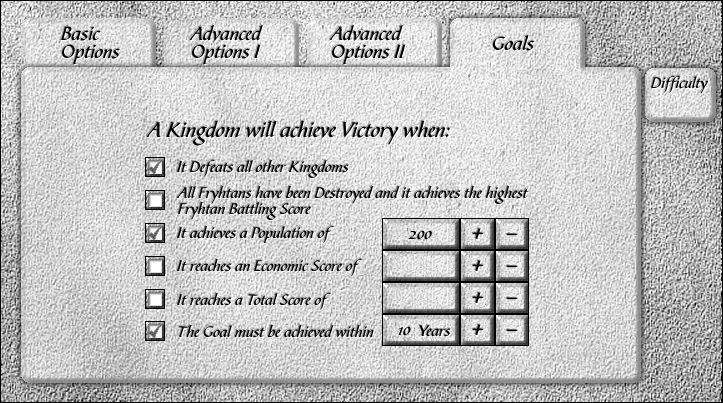
\includegraphics[width=0.9\linewidth]{Igoals}
\end{center}

On the \textbf{Goals} page, you will be able to define the victory conditions for your game. The first kingdom to achieve any of the chosen goals will be the winner.

These goals include the following:

\textbf{Defeat All Other Kingdoms}: This is not an option. Defeating all other kingdoms always results in victory, because it eliminates any possible competition for other goals. If no other goals are chosen, then victory cannot be achieved without eventually destroying all rivals, even those with whom you may have developed friendships and alliances.

\textbf{Destroy All Fryhtans}: Ridding the world of these vile creatures is a goal that all kingdoms will happily work toward. After the last of them has been destroyed, the kingdom which has dispatched the most Fryhtans will be the winner.

You may view your current score in Fryhtan Battling by \textbf{Clicking} on the Ranking Scroll at the top of your game screen.

% elipsis commonly ...

\textbf{Achieve a Population of..}: This may seem a peaceful goal, but it can often be achieved only through taking Villages by force.

\textbf{Reach an Economic Score of..}: Even the lowest possible goal here of 100 will not be achieved unless you are prepared to defend yourself and to take and hold more than one Village and, of course, to prevent your enemies from doing the same. You may check your Economic Score and the scores for the other Kingdoms by \textbf{Clicking} on the Ranking Scroll at the top of your screen and then \textbf{Clicking} on the name of the Kingdom that you want to check. Their Economic Score will appear in the box below.

\textbf{Reach a Total Score of..}: Achieving this goal requires a balanced approach to the rulership of one’s kingdom. You may check on your Total Score and that of your rivals in the same way that you checked the Economic Score.

\textbf{Achieve Goal Within..}: This will set a deadline for the achievement of the above goals.

\subsection{Winning and Losing}

\index{game!winning and losing}
\index{losing game}
\index{winning game}

\textgoth{\Huge{Y}}ou will win the game if you achieve any of the chosen goals and, if you have set a time limit, done it before that time limit is reached.

It may come to pass that, having set as your goal something other than the defeat of all of the other Kingdoms, you find a way to destroy all of your rivals anyway. Defeating all other kingdoms is always one of the goals, so you will still win the game in such a case, because the last of your competition has been eliminated.

You will lose the game if your Kingdom is destroyed, if another Kingdom has achieved a set goal, if you have failed to achieve your goal in the set time, or if you have surrender to another Kingdom.

Even though you have lost, you may continue to observe the progress of the game. The game will continue to run until you decide to either Quit or to Retire, although the score of such a game will be ineligible to be entered in the Hall of Fame.

\subsubsection{Load Game}

\index{game!loading previous saved}
\index{loading game}

\textbf{\textgoth{\Huge{C}}licking} on the Load Game Sword will take you to the Load Game menu where you can scroll up and down to see any games that you have previously saved.

\begin{center}
	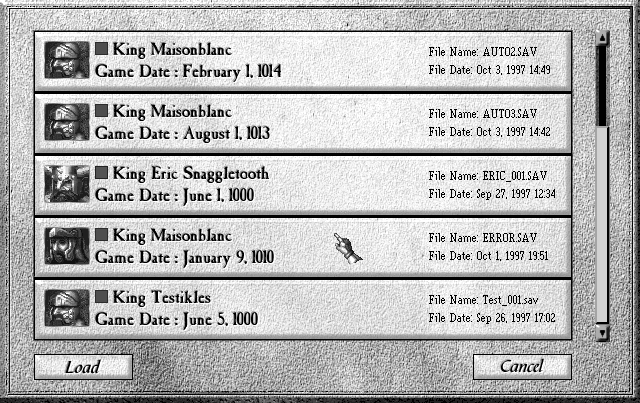
\includegraphics[width=0.9\linewidth]{Iload}
\end{center}

To load a game, \textbf{Click} on its Bar and then \textbf{Click} on the \textbf{Load Button}. You may also \textbf{Double-Click} on the Bar.

Single Player Games will have the .SAV file extension. Multiplayer Games will have the .SVM extension.

\subsubsection{Scenario}

\index{game!scenarios}
\index{scenarios}

\begin{center}
	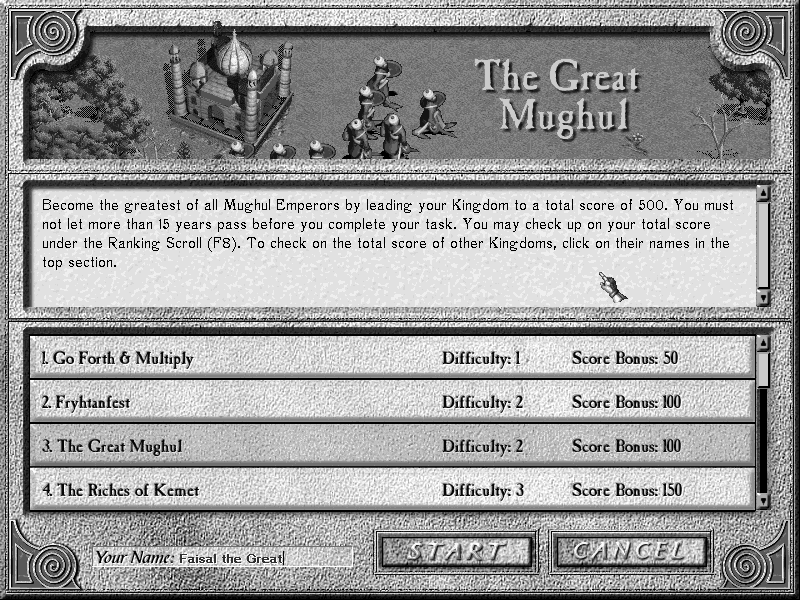
\includegraphics[width=0.9\linewidth]{Iscenario}
\end{center}

\textgoth{\Huge{C}}hoosing to play a Scenario will take you to a menu similar to the one for choosing a Training lesson. \textbf{Click} on the Scenario that you wish to play. You will see a brief description of the beginning situation and the goal(s) to be achieved. When you are ready to begin, \textbf{Click} on the \textbf{Start Button}.

\subsection{Multiplayer Game}

\index{game!multiplayer}
\index{multiplayer!game}

\begin{center}
	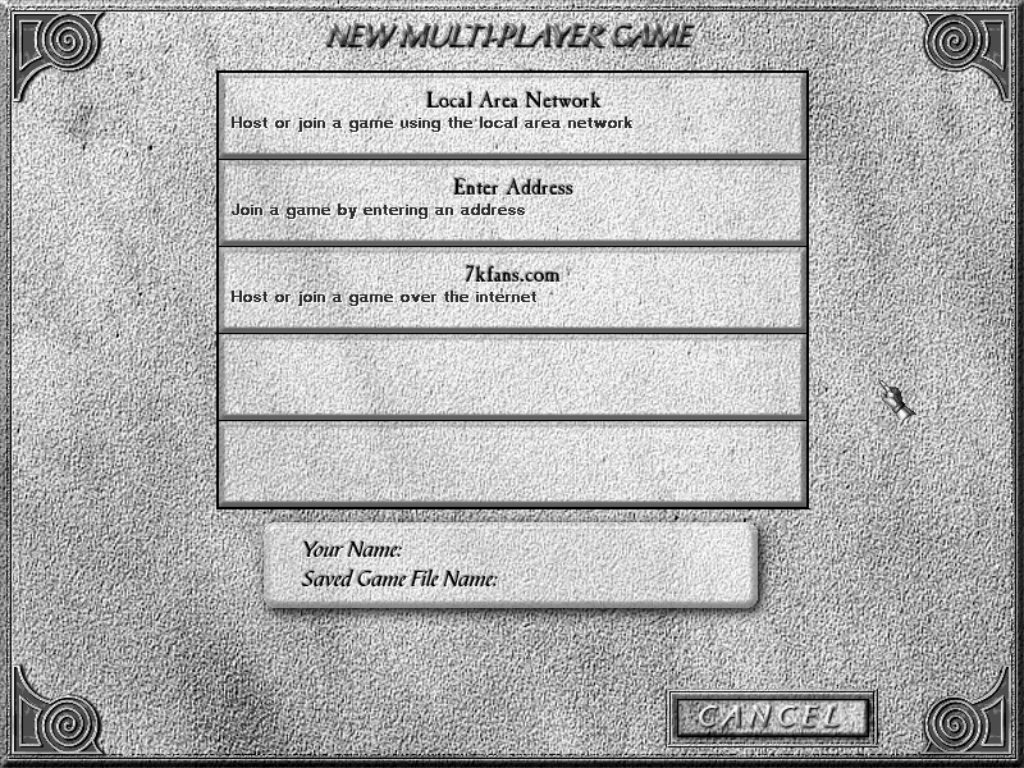
\includegraphics[width=0.9\linewidth]{Imultiplayer}
\end{center}

\subsubsection{Initial Setup} % wiki content. Author?

\textgoth{\Huge{A}}ll players need the same version of the game, or compatibility issues will arise. Allow \textit{Seven Kingdoms: Ancient Adversaries} to pass through your firewall. If you have a router, port forwarding may be needed. 2.14.7+ uses UDP port 19383 for LAN and 7kfans.com game browsing.

\subsubsection{Lobby}

\textgoth{\Huge{W}}hen you \textbf{Click} on the Multiplayer Sword you will see three connection options: Local Area Network, Enter Address (Direct IP), and 7kfans.com. \textbf{Click} on the type of connection that you will be using.

On the bottom, enter your name just as you would in a Single Player Game. This will be used by your King at the start of the game.

Beneath your name, you will see the name of the game. You will be able to save one multiplayer game only. Its name will be MULTI. You may not change this name.

There will also be two auto-saved games, named AUTO01.SVM and AUTO02.SVM. One of them will have a later date than the other, so you will know which is the most recent.

To load a saved game, Select the name of your save game file and \textbf{Click} on Load (everyone must select the same file; "Game Date" must be the same).

\subsubsection{7kfans.com}

\textgoth{\Huge{I}}f you are setting up the game, \textbf{Click} on the \textbf{Create Button}. If someone else is setting up the game, \textbf{Click} on the \textbf{Join Button}. To return to the previous screen, \textbf{Click} on the \textbf{Cancel Button}.

\begin{center}
	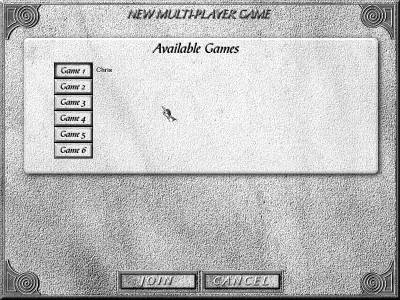
\includegraphics[width=0.9\linewidth]{Imultiplayer2}
\end{center}

If you are not creating this game, a \textbf{Click} on the \textbf{Join Button} which will send you to the Available Games page.

You will be prompted to enter your forums account username and password. If you have recently logged into the forums, you may leave your password empty.

There you will find a list of the games that have been created. They will be listed by the name the creator set. The default session name is the creator’s username. It may take a few seconds for the list of games to appear.

\textbf{Click} on the desired game’s name. Then \textbf{Click} on the \textbf{Join Button} on the bottom of the page. This will take you to the multiplayer Options pages.

\subsubsection{Enter Address}

\textgoth{\Huge{I}}f you are hosting the game, \textbf{Click} on the \textbf{Create Button}. Set the session name and choose a password. You may choose to leave the password blank. Use your external IP address to let players connect. Wait for players to join. If you are joining a game, \textbf{Click} on the \textbf{Join Button}. Enter the IP address of the host. This will take you to the multiplayer Options pages.

\subsubsection{Local Area Network}

\textgoth{\Huge{I}}f you are creating the game, \textbf{Click} on the \textbf{Create Button}. If you are joining the game, \textbf{Click} on the \textbf{Join Button}. This will take you to the multiplayer options pages.

\subsubsection{Multiplayer Options}

\textgoth{\Huge{T}}he multiplayer Options will be the same as the ones that you saw in the Single Player Options. The creator of the game sets most of the options. If you are joining a game created by someone else, you may only choose your nationality and your color.

% Graphic is right justified not centered in original.

\begin{center}
	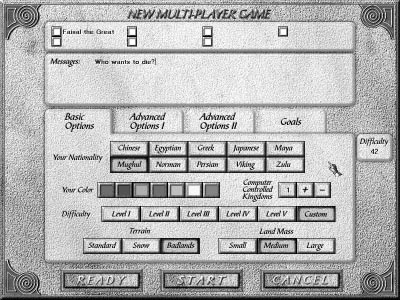
\includegraphics[width=0.9\linewidth]{Imultiplayer3}
\end{center}

The multiplayer options page includes a list of players who have joined the game, and a Chat window where players may discuss options selection, strategy, or how they intend to grind their rivals into dust. These items do not appear on the Single Player Options screen.

To send a message in the Chat window, simply type anything that you want to say. When you have finished typing, press the Enter key on your keyboard. Your message will then be posted for the other gamers to see.

Once you have set all of your options and \textbf{Clicked} on the \textbf{Ready Button}, a red check mark will appear next to your name. Do not \textbf{Click} next to your name. Nothing will happen. When every player has a red check mark visible, the creator of the game will be able to \textbf{Click} on the \textbf{Start Button} and begin the game.

\subsubsection{Matchmaking} % New content.

\textgoth{\Huge{Y}}ou can post or search on the forums to look for other players or set up matches. Look for the matchmaking thread. There are additional resources for people looking to play multiplayer such as contact information of other players.

\subsection{Encyclopedia}

\index{encyclopedia}

\begin{center}
	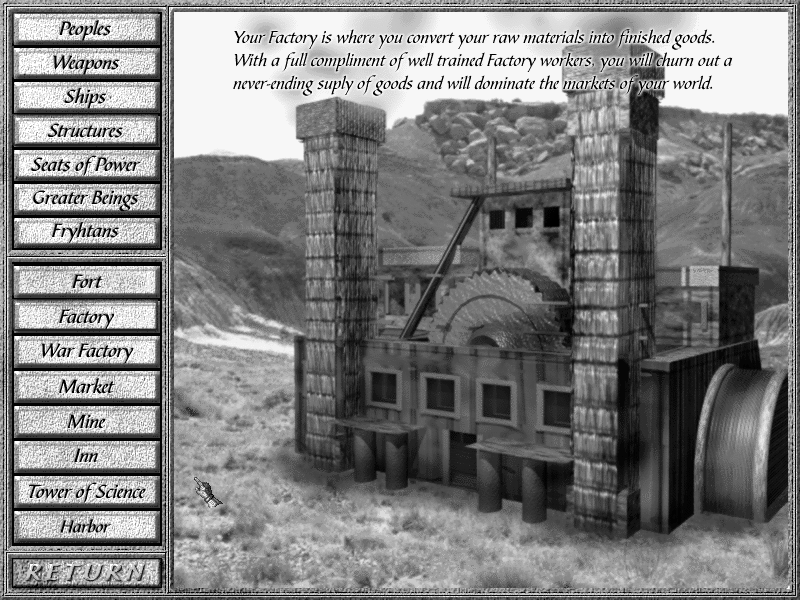
\includegraphics[width=0.9\linewidth]{Iencyclopedia}
\end{center}

\textgoth{\Huge{T}}he Encyclopedia includes images and informative descriptions of units and buildings appearing in \textit{Seven Kingdoms: Ancient Adversaries}.

\textbf{Click} on one of the titles in the top section. When you do you will see listed in the bottom section a group of subjects that are under that title.

When you \textbf{Click} on one of these you will see a picture and description of that subject.

If you do not \textbf{Click} on anything, the Encyclopedia will present you with a slideshow of all of its subjects.

\subsection{Hall of Fame}

\index{hall of fame}

\textgoth{\Huge{A}}t the end of every game of \textit{Seven Kingdoms: Ancient Adversaries} your score will be computed. Your score will take into account the difficulty level at which you were playing and the skill with which you played.

If your final score is one of the six highest ever recorded, it will be entered into the Hall of Fame.

\subsection{New Game}

\begin{wrapfigure}{r}{0.5\textwidth}
	\begin{center}
		\vspace{-20pt}
		
\includegraphics[width=0.4\textwidth]{Inewworld}
	\end{center}
\vspace{-20pt}
\end{wrapfigure}

\textgoth{\Huge{E}}very time you play a new game, a completely new world will be generated at random, giving you a nearly limitless number of worlds to subject to your will.

As soon as the new world’s lands have been separated from its waters and its mountains have been raised, you will be given a small village to call your own. From these humble beginnings you must do your best to survive and to prosper through a combination of exploration, training, construction, trade, espionage, diplomacy, and armed conflict.

You will need to develop a variety of skills to be an effective leader, and to command the loyalty of your people. Standing in your way will be other kings, evil Fryhtans, and the ravages of nature itself.

\section{Main Menu}

\index{main menu}

\textgoth{\Huge{W}}hile you are playing a game of \textit{Seven Kingdoms: Ancient Adversaries}, you will be able to access various options by \textbf{Clicking} on the \\ % FIXES AN OVERFLOW
\textbf{MENU Button} at the top right of your screen. This will bring up the options as seen below.

% Graphic is right justified not centered in original.

\begin{center}
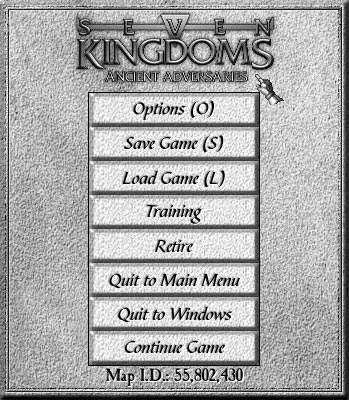
\includegraphics[width=0.5\linewidth]{Imainmenu}
\end{center}

\subsection{Options}

\textgoth{\Huge{T}}he first choice you will have, which can also be accessed by pressing the O key on your keyboard, is the In-game Options Page.

\begin{center}
	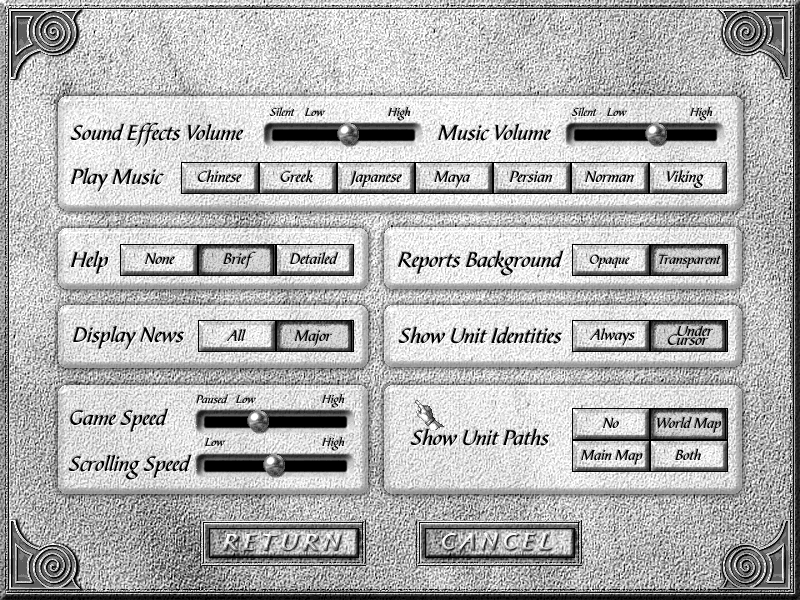
\includegraphics[width=0.9\linewidth]{Ioptions}
\end{center}

Here you can set your Sound Effects and Music volume. Do this by sliding the brass ball left or right until it is in the position that you want.

You may also choose to play any single piece of \textit{Seven Kingdoms: Ancient Adversaries} music.

You can set the detail level of pop-up instructional text that will appear whenever you hold the cursor over a button or icon for a few seconds. You may also turn this feature off, if you prefer.

You can choose to view all News items or only the most important ones.

You can set the Speed of the game (which can also be set on your keyboard by pressing the 0–-9 keys at any time) and the Scrolling Speed of your screen.

For your Reports Background you have the option of seeing through them to any action that is taking place (transparent), or the option of making them opaque.

Unit Identities (what kind of skills units possess) can be set to be seen at all times or only when a unit is under your cursor.

Finally, you may whether to display the projected Paths that your units will take when they have been ordered to move to a different part of the map.

\subsubsection{Help}

\index{help}

\textgoth{\Huge{T}}o use the Help function, simply hold your cursor over any button or icon in the game. After a few seconds, a display will appear explaining the use of the button or meaning of the icon. You may set the detail level of this Help function on the Options Page (O), or disable it if you prefer.

Because the Help function pauses the game momentarily to allow you time to read, it will not be available in multiplayer games.

\subsection{Save Game}

\index{game!saving}
\index{saving game}

\textgoth{\Huge{I}}f you choose Save Game, you will be presented with a screen showing all of the games that have previously been saved. You may choose to overwrite any one of these games by \textbf{Clicking} on the game’s name and then \textbf{Clicking} on the \textbf{Save Button}.

\begin{center}
	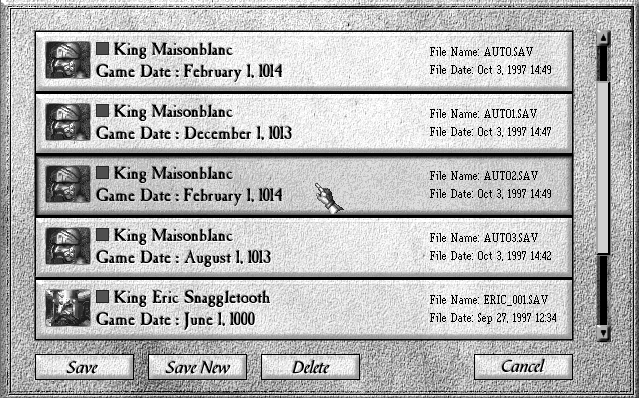
\includegraphics[width=0.9\linewidth]{Isavegame}
\end{center}

You may also choose to save your game in a new file by \textbf{Clicking} on the \textbf{Empty Game Slot Button}, which will be at the very top of the list, and then on the \textbf{Save New Button}.

\begin{center}
	
\includegraphics[width=0.7\linewidth]{Isavegame_emptyslot}
\end{center}

Although the number of games that you can save is limited only by your disk space, you may wish to delete some of your more humiliating defeats. To do so, \textbf{Click} on the game and then \textbf{Click} on the \textbf{Delete Button}.

The game that you are playing will be automatically saved in a separate file after every two months of game time. Auto-saved games will have filenames beginning with AUTO.

\subsection{Retire}

\index{retiring}

\textgoth{\Huge{W}}hen you decide to retire from a game of \textit{Seven Kingdoms: Ancient Adversaries}, the game will end and your score will be calculated.

If you have achieved a high enough score, it will be entered in the Hall of Fame.

If you choose to Retire from a multiplayer game, the computer will take control of your kingdom and do its best to finish on top.

\subsection{Map I.D.}

\index{map ID}

\textgoth{\Huge{T}}he Map I.D. is the random number seed from which your present world map was generated. Make a note of this number if you particularly like a random map and would like to use it again, share it with your friends, or post on the Internet.

\section{Mouse and Keyboard Commands and Cheat Codes}

% I think one or two is missing: new kingdom emerge, replay.

\subsection{Mouse Commands}

\index{mouse commands}

\begin{center}
	\begin{tabular}{|p{2in}|p{2in}|}
		\hline
		Action	& Description \\ \hline
		Click	& Press the left mouse button once. \\ \hline
		Double-Click	& Press the left mouse button twice quickly. \\ \hline
		Right-Click	& Press the right mouse button once. \\ \hline
		Group Select	& Click and hold down the left mouse button, dragging a box around the intended group. \\ \hline
		Right-Click on town transfer	& Transfers 10 peasants \\ \hline
		Right-Click on research project	& Sets research project for all towers of science \\ \hline
		Right-Click on train unit	& Dequeue 8 units \\ \hline
		Right-Click on collect tax	& Set automatic tax \\ \hline
		Right-Click on grant	&  Set automatic grant \\
		\hline
	\end{tabular}
\end{center}

\clearpage

\subsection{Keyboard Commands}

\index{hotkeys}
\index{keyboard shortcuts}

\begin{center}
	\begin{tabular}{|p{1in}|p{3in}|}
		\hline	 
		Action	& Description \\ \hline
		Esc	& Close Scroll Reports. \\ \hline
		F1	& Kingdoms report \\ \hline
		F2	& Villages report \\ \hline
		F3	& Economy report \\ \hline
		F4	& Trade report \\ \hline
		F5	& Military report \\ \hline
		F6	& Technology report \\ \hline
		F7	& Espionage report \\ \hline
		F8	& Ranking report \\ \hline
		F9	& View the News Log. \\ \hline
		F11	& Capture the Screen to a .BMP file. The screenshot will be saved in the game’s directory. \\ \hline
		0 (zero) & Pause the Game. Many overlays and menus will still be operational even while the game is paused. Units can be given new orders, but they will carry them out when the game is resumed. \\ \hline
		1--9 & Set the Speed of the Game. 1 is the slowest---and 9 the fastest. \\ \hline
		Spacebar & Pause/unpause the game. \\ \hline
		Shift + Right-Click	& Queue 8 units / queue 10 weapons / queue 4 ships \\ \hline
		Up / Down Arrows & Go to the previous/next building of the same type as the currently selected one. \\ \hline
		Left / Right Arrows	& Go to the previous/next object of the same type and of the same nationality as the currently selected one. \\ \hline
		b & If you select a unit, it will give you the build command. If you select a town, it will give you the train command. \\ \hline
		b+a	& Build a factory \\ \hline
		b+f	& build a fort \\ \hline
		b+h	& build a harbor \\ \hline
		b+i	& build an inn \\ \hline
		b+m	& build a market \\ \hline
		b+p	& build a seat of power \\ \hline
		b+r	& build a mine \\ \hline
		b+t	& build a tower of science \\ \hline
	\end{tabular}
\end{center}

\begin{center}
	\begin{tabular}{|p{1in}|p{3in}|}
		\hline	 	
		Action	& Description \\ \hline
		d	& Open first diplomacy message / reply to chat \\ \hline
		e	& Switch the World Map Display Modes. \\ \hline
		f	& Select a Fort and center the screen on it. Press repeatedly to cycle through all of your Forts. Pressing the left or right arrow keys will also cycle through your Forts. Pressing the up and down arrow keys will cycle through all Forts, including those of other Kingdoms. \\ \hline
		g	& Select a General and center the screen on him. Press repeatedly to cycle through all of your Generals. \\ \hline
		u	& Select a Ship and center the screen on it. Press repeatedly to cycle through all of your Ships. \\ \hline
		j	& Center the screen on the location of a Natural Resource deposit. \\ \hline
		k	& Select your King and center the screen on him. \\ \hline
		l (el)	& Load a Game. \\ \hline
		o (oh)	& In-Game Options Menu. \\ \hline
		p	& Toggle between Opaque and Transparent Reports. \\ \hline
		r	& If you select a fort, it will Sortie the soldiers. If you select soldiers, it will withdraw them. If you select a village, it will recruit peasants. \\ \hline
		s	& Save the Game. The game will be Auto-Saved every two months in a separate file. \\ \hline
		t	& Settle \\ \hline
		x	& Clear all News and / or Chat messages from the screen. \\ \hline
		y	& Select a Spy and center the screen on him. Press repeatedly to cycle through all of your Spies. \\ \hline
	\end{tabular}
\end{center}	

\begin{center}
	\begin{tabular}{|p{1in}|p{3in}|}
		\hline	 	
		Action	& Description \\ \hline
		\textgreater & Next block of text in Training. \\ \hline
		\textless	& Previous block of text in Training. \\ \hline
		Ctrl + (0--9)	& Assign all selected units to a numbered group. \\ \hline
		Alt + (0--9)	& Select all mobile units previously assigned to a numbered group. \\ \hline
		Alt + Right-Click	& Manually assign waypoints to mobile unit(s). After setting waypoints, use a normal Right Click to set the final destination. \\ \hline
		Alt + Enter & Enter or leave windowed mode \\ \hline
		Alt + g & Screen grab in windowed mode \\ \hline
		Alt + F4	& Quit to Desktop \\ \hline
	\end{tabular}
\end{center}

\subsection{Cheat Codes}

\index{cheats}

\textgoth{\Huge{T}}ype !!!@@@\#\#\# during gameplay to enable cheat mode. Note that the game will say you cheated, and your score will be zero.

\begin{center}
	\begin{tabular}{|p{1in}|p{3in}|}
		\hline	 
		Action	& Description \\ \hline
		c	& Add \$1000 \\ \hline
		n	& Add all technology \\ \hline
		u	& Enable / disable King immortal mode. \\ \hline
		z	& Construct building instantly \\ \hline
		=	& Fill prayer bar in seat of power \\ \hline
		[	& +20 combat skill \\ \hline
		]	& +20 skill \\ \hline
		;	& +10 population \\ \hline
		‘	& +20 spy skill \\ \hline
		\textbackslash & Add 1000 food \\ \hline
		/	& Reveal map \\ \hline
	\end{tabular}
\end{center}